%!TeX root=MemoriaTFG.tex

\chapter{Project management}\label{chap:management}

\section{Origin of the project}

The project began with a search for a practical problem that had not been solved satisfactorily for non-technical users. I considered several possible applications based on difficulties I had encountered myself or heard about from other people. The idea for Wave Launcher appeared when acquaintances asked me for help setting up a Minecraft server because they could not complete the process on their own. No single step was especially obscure. The difficulty came from having to combine a server distribution, a suitable Java runtime, configuration files, a mod loader, compatible mods and router settings. This experience gave the project both a concrete target user and a useful objective.

An initial technology study was carried out before a tutor was sought. C\# was selected partly because the project offered an opportunity to improve existing knowledge of the language. A multi-platform user interface was also an early objective, which led to the selection of .NET MAUI. The first release was nevertheless scoped to Windows because this is where most casual Minecraft: Java Edition players use the game. It was also the platform available for development and testing. MAUI preserves the possibility of reusing the interface on other platforms, but supporting them was not part of the completed scope because process execution and device-information access would require additional platform-specific implementations.

Before formally committing to the topic, a one-month feasibility period was used to explore the framework, the available provider interfaces and the likely complexity of the server-management operations. At the end of that period, the project was considered feasible and development continued as the final degree project.

This exploratory beginning was useful because several external dependencies were not under the project's control. Mojang, Eclipse Adoptium, Forge, Fabric, Modrinth and CurseForge each publish different data and use different release models. Confirming that enough metadata could be obtained was necessary before a graphical workflow could be promised. The feasibility work also showed that the program could own its Java installations and server files instead of depending entirely on software configured elsewhere on the computer.

\section{Development method}

Development followed an iterative and incremental process. At the start of each working week, I selected a milestone that seemed achievable in approximately 10 to 20 hours. Each milestone had a concrete result, such as defining a group of ports, integrating an external catalogue, implementing a management operation or completing a user-interface workflow. Small or familiar tasks, particularly integrations similar to one already completed, were grouped together. Less predictable work was given a complete iteration.

The process was deliberately lightweight because the project had one developer. A Scrum process would have introduced ceremonies and roles that could not serve their normal purpose in a one-person project. Instead, the weekly milestone provided a short feedback cycle without pretending that a team process was being followed. The high-level schedule was represented in a Gantt diagram, while daily work was tracked with the Todo Tree extension for Visual Studio Code. Todo Tree collected pending interfaces, services, defects and general improvements directly from annotations in the source tree.

\begin{figure}[htbp]
  \centering
  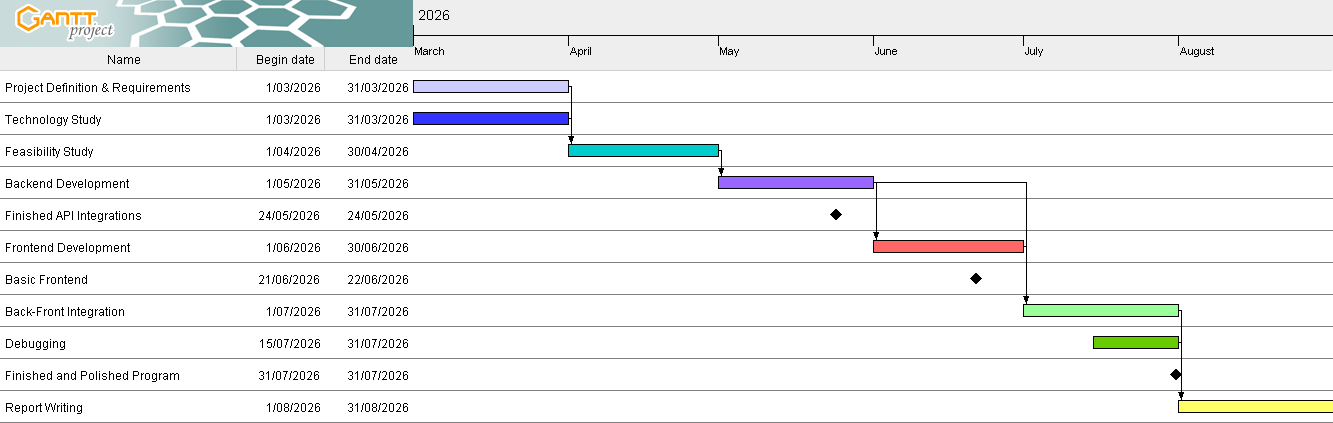
\includegraphics[width=\textwidth,height=0.72\textheight,keepaspectratio]{Gantt.png}
  \caption{High-level Gantt diagram of the project phases.}
  \label{fig:gantt}
\end{figure}

The Gantt plan separated the work into project definition and requirements, technology study, back-end implementation, user-interface implementation, integration and correction, and report writing. Notes for the report were collected throughout development so that design decisions and implementation difficulties would not have to be reconstructed only at the end. Git and GitHub were used for version control and remote backup. No branching strategy was necessary for a single developer; a commit was normally pushed after a significant milestone had reached a stable state.

\section{Phases and evolution}

\subsection{Project and architecture setup}

The first implementation phase established the solution and its C\# projects. The user interface, application contracts, infrastructure implementations and domain model were separated from the beginning. This setup took approximately two weeks because both .NET MAUI and the architectural style were new in practice. Much of the time was consequently spent learning how MAUI applications are composed, how dependencies cross project boundaries and how asynchronous operations should be exposed to view models.

Starting with boundaries rather than concrete integrations had a direct effect on later work. The interfaces in the application project described the operations needed by the functional requirements, and the infrastructure project could then implement those contracts with file-system, process and HTTP details. It was still possible to revise a contract when the interface revealed a missing use case, but provider-specific data did not become the public vocabulary of the complete application.

\subsection{Services and external integrations}

After the project structure was stable, the input services and output ports were defined. This stage lasted approximately three months and included the study and integration of the external sources. Java distribution required more investigation than initially expected. Microsoft OpenJDK was considered, but it did not provide the catalogue interface needed by the application, so the supported suppliers were limited to Eclipse Adoptium and Mojang. Both major mod platforms, Modrinth and CurseForge, provide APIs and were therefore selected. Fabric exposes a documented catalogue. Forge required additional investigation because the needed version information is obtained from its Maven metadata rather than from a dedicated public REST API.

Hoppscotch was used during this phase to inspect HTTP responses and understand provider data. Some orchestration behavior, particularly complete migration of a server and its mods, was postponed until a user interface existed. Exercising a long stateful workflow through isolated HTTP and service calls would have made diagnosis unnecessarily difficult. The interfaces and the basic operations were implemented first, then the postponed behavior was completed when it could be driven and observed through the application.

\subsection{User-interface implementation}

The user interface was developed during June 2026. The first version was intentionally rudimentary. Its purpose was to expose every functional workflow and reveal whether the service contracts contained the information required by a real interaction. This phase confirmed that the back end and front end could not be developed as two strictly consecutive products. Several services evolved when the screens made the order of selections, validation needs and change summaries concrete.

By early July the functional requirements were accessible through the interface. The remainder of July was assigned to visual refinement, clearer feedback and edge-case testing. Form controls generated most of the unexpected work. Their MAUI behavior did not always match the assumptions made in the first reusable form implementation, so binding, selection and validation logic required revision. These corrections extended the final defect-removal phase by approximately one week into early August. This was the only material deviation from the high-level schedule.

\section{Risk management}

The planning process did not maintain a separate formal risk register, but several technical risks influenced the order of work. External provider changes were the main risk. The application cannot control the structure, availability or authentication rules of remote catalogues. Provider access was therefore placed behind ports and mapped into domain objects. A change to one supplier should remain localized to its adapter unless it changes the meaning of the domain information.

Framework uncertainty was another risk because the project began without prior MAUI experience. Unexpected limitations in binding, navigation or native control behavior could have forced extensive changes after the application services were already implemented. The early feasibility month and the initial architecture phase reduced this risk before most application behavior was built. The final form-control problems described in the previous section show that the risk did materialize to a limited extent, producing a one-week delay rather than requiring a change of framework.

Server migration presented a risk of leaving an instance unusable or losing installed components. A new Minecraft version may not have a compatible release of the existing mod loader or every installed mod, and a download can fail after earlier files have already been changed. To reduce this risk, the migration workflow evaluates dependent components, shows the expected changes before confirmation and reports mods that were removed, required, incompatible or could not be downloaded. Its implementation was postponed until the interface could expose those consequences clearly. The remaining risk is that file-system changes are not performed as one atomic transaction, so an interruption at the wrong point can still leave a partly modified directory. Chapters~\ref{chap:design} and~\ref{chap:implementation} describe this limitation and the proposed use of staged updates and backups.

\section{Assessment of the process}

Weekly milestones were a good fit for exploratory integration work. They provided a definition of progress that was more meaningful than time spent, and they allowed knowledge gained from one provider to improve the next integration. The approach also made it possible to change service contracts during interface development without invalidating a large plan of detailed tasks.

The process had two limitations. First, the 10 to 20 hour weekly range was an estimate rather than recorded time, so it cannot support an exact cost calculation. Second, the absence of a detailed historical backlog means that the final sequence can only be reported at phase and milestone level. For a future team project, a shared Kanban board and a Scrum-style iteration review would provide better coordination and a more auditable history. For this individual project, the combination of a Gantt overview, source annotations and milestone commits was sufficient to keep the implementation directed toward the functional scope.
